%----------------------------------------------------------------------------------------
%	PACKAGES AND OTHER DOCUMENT CONFIGURATIONS
%----------------------------------------------------------------------------------------

\documentclass[
11pt, % Main document font size
a4paper, % Paper type, use 'letterpaper' for US Letter paper
oneside, % One page layout (no page indentation)
headinclude,footinclude, % Extra spacing for the header and footer
BCOR5mm, % Binding correction
]{scrartcl}


%----------------------------------------------------------------------------------------
%	REQUIRED PACKAGES
%----------------------------------------------------------------------------------------

\usepackage[
nochapters, % Turn off chapters since this is an article        
beramono, % Use the Bera Mono font for monospaced text (\texttt)
eulermath,% Use the Euler font for mathematics
pdfspacing, % Makes use of pdftex’ letter spacing capabilities via the microtype package
dottedtoc % Dotted lines leading to the page numbers in the table of contents
]{classicthesis} % The layout is based on the Classic Thesis style

\usepackage{arsclassica} % Modifies the Classic Thesis package

\usepackage[T1]{fontenc} % Use 8-bit encoding that has 256 glyphs

\usepackage[utf8]{inputenc} % Required for including letters with accents

\usepackage{graphicx} % Required for including images
\graphicspath{{Figures/}} % Set the default folder for images

\usepackage{enumitem} % Required for manipulating the whitespace between and within lists

\usepackage{lipsum} % Used for inserting dummy 'Lorem ipsum' text into the template

\usepackage{subfig} % Required for creating figures with multiple parts (subfigures)

\usepackage{amsmath,amssymb,amsthm} % For including math equations, theorems, symbols, etc

\usepackage{varioref} % More descriptive referencing

%----------------------------------------------------------------------------------------
%	THEOREM STYLES
%---------------------------------------------------------------------------------------

\theoremstyle{definition} % Define theorem styles here based on the definition style (used for definitions and examples)
\newtheorem{definition}{Definition}

\theoremstyle{plain} % Define theorem styles here based on the plain style (used for theorems, lemmas, propositions)
\newtheorem{theorem}{Theorem}

\theoremstyle{remark} % Define theorem styles here based on the remark style (used for remarks and notes)

%----------------------------------------------------------------------------------------
%	HYPERLINKS
%---------------------------------------------------------------------------------------

\hypersetup{
%draft, % Uncomment to remove all links (useful for printing in black and white)
colorlinks=true, breaklinks=true, bookmarks=true,bookmarksnumbered,
urlcolor=webbrown, linkcolor=RoyalBlue, citecolor=webgreen, % Link colors
pdftitle={}, % PDF title
pdfauthor={\textcopyright}, % PDF Author
pdfsubject={}, % PDF Subject
pdfkeywords={}, % PDF Keywords
pdfcreator={pdfLaTeX}, % PDF Creator
pdfproducer={LaTeX with hyperref and ClassicThesis} % PDF producer
} % Include the structure.tex file which specified the document structure and layout
\usepackage{abstract}
\hyphenation{Fortran hy-phen-ation} % Adds hyphenation for cut off words

%Interactive links and table of contents
\hypersetup{
    colorlinks=true, 
    linktoc=all,    
    linkcolor=black,
    urlcolor=blue,
}

%Packages:
\hypersetup{breaklinks=true}
\urlstyle{same}
\usepackage{color}   
\usepackage{etoolbox}
\usepackage{sectsty}
\sectionfont{\fontsize{15}{15}\selectfont}
\usepackage{float}
\usepackage{authblk}
\usepackage{titling}

%Redefining Abstract
\renewenvironment{abstract}
 {\quotation\small\noindent\rule{\linewidth}{.5pt}\par\smallskip
  {\centering\bfseries\abstractname\par}\medskip}
 {\par\noindent\rule{\linewidth}{.5pt}\endquotation}
\usepackage{geometry}

%Changes Margins
 \geometry{
 a4paper,
 left=25mm,
 right=25mm,
 top=25mm,
 bottom = 20mm,
 headsep = 9mm,
 }
%https://www.overleaf.com/learn/latex/Page_size_and_margins for more control overlayout
%----------------------------------------------------------------------------------------
%	TITLE AND AUTHOR(S)
%----------------------------------------------------------------------------------------
\title{\normalfont\spacedallcaps{Python Graphing: 3D Contour Plots}\vspace{-0.4in}} % The article title
\author{\small\\\textbf{Author: }Javier Huang\\
        \vspace*{0.05in} %Adds small space between 2 text or could be used to subtract space
        \textbf{Editor: }Jim Chen\\
        \vspace*{-0.1in} \\ 
	    \textbf{Date Created: }06/10/23\\
	    \vspace*{0.05in}
	    \textbf{Date Edited: }06/10/23\\
	    \vspace*{0.05in}
	    Version 1.0
       }
\date{\vspace{-5ex}} %Removes date function
%----------------------------------------------------------------------------------------

\begin{document}

%----------------------------------------------------------------------------------------
%	HEADERS
%----------------------------------------------------------------------------------------

\ohead{


    \mbox{\large\rightmark\hspace{0.8em}\rlap{\vline\kern1em\pagemark}} %Page number and the line separation 
}
\addtokomafont{pagenumber}{\small}
\addtokomafont{pagehead}{\color{black}}

\renewcommand{\sectionmark}[1]{\markright{\spacedlowsmallcaps{~#1}}}

\pagestyle{scrheadings} % Enable the headers specified in this block
%----------------------------------------------------------------------------------------
%	ABSTRACT & TITLE
%----------------------------------------------------------------------------------------
\begin{figure} %This H sets the position for the images. Since latex images are floats, latex usually puts them in the best spot unless you use this 
\centering 

\includegraphics[scale=0.15]{Figures/caypt_logo.jpg}\vspace{-1in}
\end{figure}
\maketitle % Print the title/author/date block
\begin{abstract}\centering\noindent %Adds center aligned text and no indents
In this SOP, the principle of graphing 3D contour plots in the Python programming language is documented.
\end{abstract}
\vspace*{0.15in}
\begin{figure}
\centering %Centering image
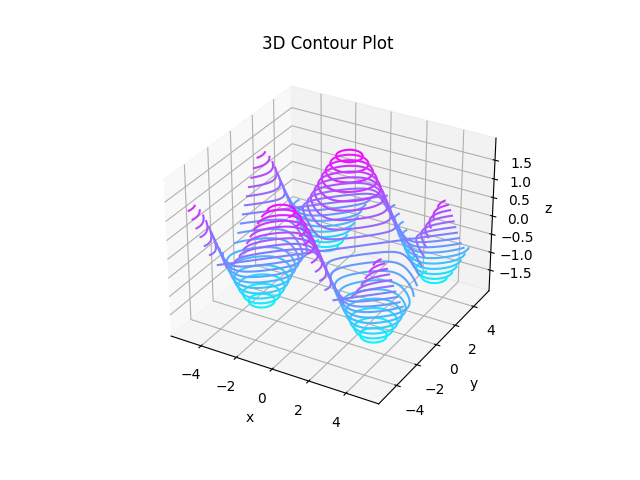
\includegraphics[width=0.6\columnwidth]{Figures/Figure0.png} %adding images
\end{figure}
%----------------------------------------------------------------------------------------
%	TABLE OF CONTENTS & LISTS OF FIGURES AND TABLES
%----------------------------------------------------------------------------------------

\makeatletter
\pretocmd{\chapter}{\addtocontents{toc}{\protect\addvspace{0\p@}}}{}{} %Controls spacing between table of contents
\pretocmd{\section}{\addtocontents{toc}{\protect\addvspace{7\p@}}}{}{}
\pretocmd{\subsection}{\addtocontents{toc}{\protect\addvspace{5\p@}}}{}{}
\makeatother

\setcounter{tocdepth}{2} %set the depth of the table of contents to show sections and subsections only 

\pagebreak
\tableofcontents % Print the table of contents
\listoffigures % Print the list of figures

%\listoftables % Print the list of tables

%----------------------------------------------------------------------------------------
%	Footnotes
%----------------------------------------------------------------------------------------

%\let\thefootnote\relax\footnotetext{\textsuperscript{1} \textit{Footnote 1 etc.}}

%\let\thefootnote\relax\footnotetext{\textsuperscript{2} \textit{Footnote 2 etc.}}

%----------------------------------------------------------------------------------------

\newpage % Start the article content on the second page, remove this if you have a longer abstract that goes onto the second page

%----------------------------------------------------------------------------------------
%	INTRODUCTION
%----------------------------------------------------------------------------------------

\section{Uses of 3D Contour Graphing}
%A statement requiring citation \cite{Figueredo:2009dg}.
A contour plot is a useful visualization technique that allows us to explore the potential relationship between three variables by representing the 3-dimensional relationship in two dimensions. It involves plotting the x-axis and y-axis variables (often referred to as predictors) on the corresponding scales, while the response values (z) are represented by contours.\cite{Minitab}
\newline
\newline
3D contour plots are commonly used to visualize physical phenomena including:

\begin{enumerate}
	\item Gravitational Potential
	\begin{enumerate}
		\item[] 3D contour plots serve as a valuable tool for visualizing the gravitational potential in a given region of space.
	\end{enumerate}
	\item Electric and Magnetic Fields
	\begin{enumerate}
		\item[] By graphically depicting field strengths at different points in space, 3D contour plots facilitate the visualization of field patterns and the identification of areas featuring stronger or weaker fields.
	\end{enumerate}
	\item Temperature Distributions
	\begin{enumerate}
		\item[] 3D contour plots are constructed by mapping temperature values onto a three-dimensional grid, which allow for the visualization of temperature variations and gradients, thereby aiding in the analysis of heat transfer processes.
	\end{enumerate}
\end{enumerate}
%----------------------------------------------------------------------------------------
%	Python installation
%----------------------------------------------------------------------------------------
\section{Installing the Python packages}
\begin{enumerate}
	\item Open the Integrated Development Environment (IDE). This SOP will focus on using Visual Studio Code (VSCode).
	\item Go to the Terminal section of VSCode (Fig. 1) or open the Windows Command Prompt (Fig. 2).
	\begin{figure}[H]
		\centering %A statement requiring citation \cite{Figueredo:2009dg}
		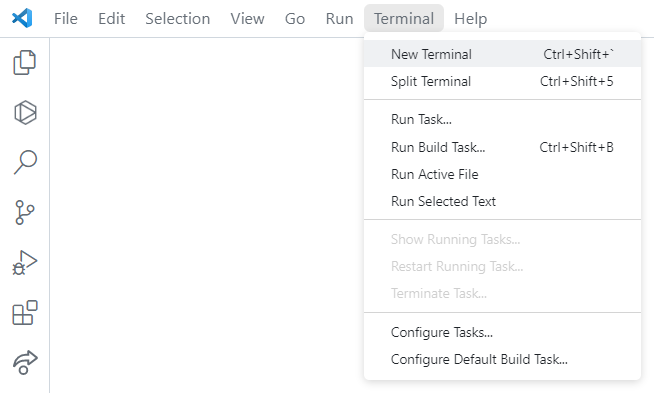
\includegraphics[width=0.4\columnwidth]{Figures/Figure1.png} 
		\caption[VSCode Terminal]{VSCode Terminal} % The text in the square bracket is the caption for the list of figures while the text in the curly brackets is the figure caption
		\label{fig:gallery} 
	\end{figure}
	\begin{figure}[H]
		\centering %A statement requiring citation \cite{Figueredo:2009dg}
		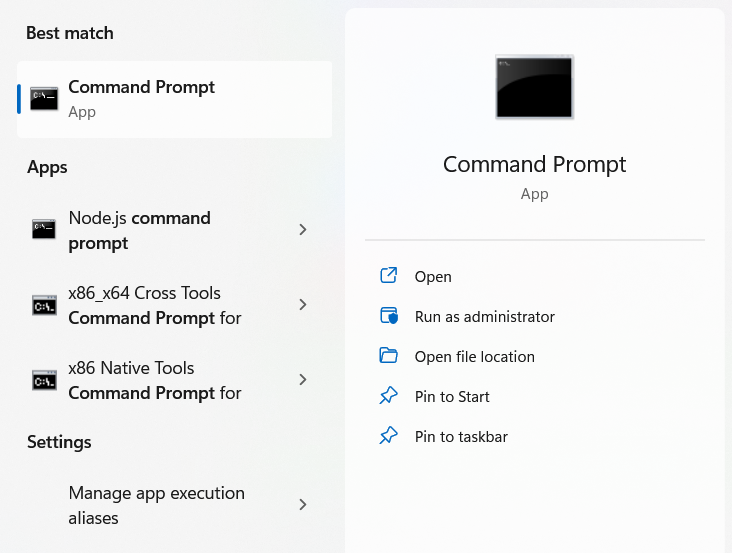
\includegraphics[width=0.4\columnwidth]{Figures/Figure2.png} 
		\caption[Command Prompt]{Command Prompt} % The text in the square bracket is the caption for the list of figures while the text in the curly brackets is the figure caption
		\label{fig:gallery} 
	\end{figure}
	\item The graphing requires two packages, NumPy and MatPlotLib. To install them, type in the following commands separately to either the VSCode Terminal or the Command Prompt Terminal
	\begin{enumerate}
		\item[] \begin{verbatim}
			pip install numpy
		\end{verbatim}
		\item[] \begin{verbatim}
			pip install matplotlib
		\end{verbatim}
	\end{enumerate}
\end{enumerate}

%----------------------------------------------------------------------------------------
%	CODE
%----------------------------------------------------------------------------------------

\section{Graphing a 3D Contour Plot with Examples}

\subsection{Creating a Generic Function Plot}
	\begin{enumerate}
		\item Create a new Python file, and import the libraries
		\begin{enumerate}
			\item[] \begin{verbatim}
				from mpl_toolkits import mplot3d
				import numpy as np
				import matplotlib.pyplot as plt
			\end{verbatim}
		\end{enumerate}
		\item Generate the data for the contour plot. You can use NumPy to create a grid of x, y, and z values. In this example, we'll create a grid ranging from -5 to 5 for both x and y, and use the function $\sin(\sqrt{x^2 + y^2})$ for the z
		\begin{enumerate}
			\item[] \begin{verbatim}
				# Define the function to be plotted
				def f(x, y):
				    return np.sin(np.sqrt(x ** 2 + y ** 2))

				# Generate x and y values
				x = np.linspace(-5, 5, 100)
				y = np.linspace(-5, 5, 100)

				# Create a grid of x and y values
				X, Y = np.meshgrid(x, y)

				# Evaluate the function for each combination of x and y
				Z = f(X, Y)
			\end{verbatim}
		\end{enumerate}
		\item Plot the contour plot by passing the x, y, and z values, along with the number of contour levels (20) and the desired colormap
		\begin{enumerate}
			\item[] \begin{verbatim}
				# Create a new figure
				fig = plt.figure()

				# Create a 3D axes object
				ax = plt.axes(projection='3d')

				# Create a 3D contour plot
				ax.contour3D(X, Y, Z, 20, cmap='jet')
			\end{verbatim}
		\end{enumerate}
		\item Add labels and customize the plot if desired
		\begin{enumerate}
			\item[] \begin{verbatim}
				# Set labels for x, y, and z axes
				ax.set_xlabel('x')
				ax.set_ylabel('y')
				ax.set_zlabel('z')
			\end{verbatim}
		\end{enumerate}
		\item Display the plot
		\begin{enumerate}
			\item[] \begin{verbatim}
				# Display the plot
				plt.show()
			\end{verbatim}
		\end{enumerate}
		\item Finally, execute the code to see the contour plot open in a separate window
	\end{enumerate}
	
	\textbf{Complete code for graphing a 3D contour plot in Python:}

	\begin{verbatim}
		import numpy as np
		from mpl_toolkits import mplot3d
		import matplotlib.pyplot as plt
		
		# Define the function to be plotted
		def f(x, y):
		    return np.sin(np.sqrt(x ** 2 + y ** 2))
		
		# Generate x and y values
		x = np.linspace(-5, 5, 100)
		y = np.linspace(-5, 5, 100)
		
		# Create a grid of x and y values
		X, Y = np.meshgrid(x, y)
		
		# Evaluate the function for each combination of x and y
		Z = f(X, Y)
		
		# Create a new figure
		fig = plt.figure()
		
		# Create a 3D axes object
		ax = plt.axes(projection='3d')
		
		# Create a 3D contour plot
		ax.contour3D(X, Y, Z, 20, cmap='jet')
		
		# Set labels for x, y, and z axes
		ax.set_xlabel('x')
		ax.set_ylabel('y')
		ax.set_zlabel('z')
		
		# Set the title of the plot
		ax.set_title('3D Contour Plot')
		
		# Display the plot
		plt.show()
	\end{verbatim}
	\textbf{The output of the program is displayed in Fig. 3}
	
	\begin{figure}[H]
		\centering %A statement requiring citation \cite{Figueredo:2009dg}
		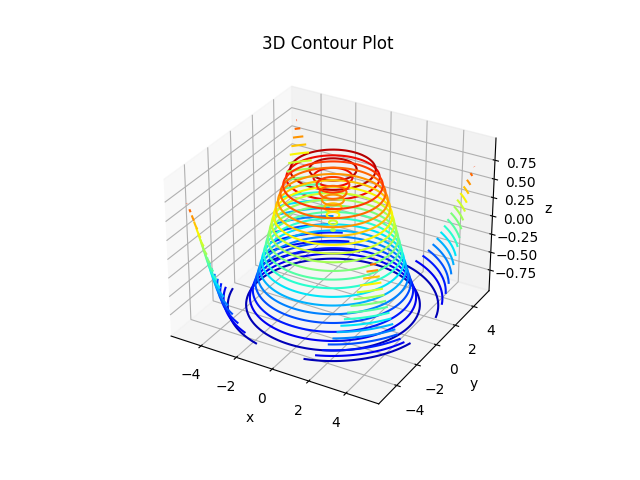
\includegraphics[width=0.4\columnwidth]{Figures/Figure3.png} 
		\caption[Final Generic 3D Contour Plot]{Final Generic 3D Contour Plot} % The text in the square bracket is the caption for the list of figures while the text in the curly brackets is the figure caption
		\label{fig:gallery} 
	\end{figure}
	
\subsection{Creating a Physics Related Plot}
	
	The following example displays the gravitational potential of a point mass.
	\newline
	\newline
	The function used in the plot is:
	\begin{enumerate}
		\item[] \begin{verbatim}
			# Gravitational constant
			G = 6.67430e-11
			
			# Define the gravitational potential function for a point mass
			def gravitational_potential(x, y, mass):
			    r = np.sqrt(x ** 2 + y ** 2)  # Distance from the origin
			    return -G * mass / r
		\end{verbatim}
	\end{enumerate}
	\textbf{Complete code for creating a physics related 3D contour plot in Python:}
	\begin{verbatim}
		import numpy as np
		from mpl_toolkits import mplot3d
		import matplotlib.pyplot as plt
		
		# Gravitational constant
		G = 6.67430e-11
		
		# Define the gravitational potential function for a point mass
		def gravitational_potential(x, y, mass):
		    r = np.sqrt(x ** 2 + y ** 2)  # Distance from the origin
		    return -G * mass / r
		
		# Generate x, y, and z values
		x = np.linspace(-5, 5, 100)
		y = np.linspace(-5, 5, 100)
		
		# Create a grid of x, y, and z values
		X, Y = np.meshgrid(x, y)
		
		# Define the mass of the point mass
		mass = 1
		
		# Evaluate the gravitational potential function for each combination of x, y, and z
		Z = gravitational_potential(X, Y, mass)
		
		# Create a new figure
		fig = plt.figure()
		
		# Create a 3D axes object
		ax = plt.axes(projection='3d')
		
		# Create a 3D contour plot
		ax.contour3D(X, Y, Z, 50, cmap='jet')
		
		# Set labels for x, y, and z axes
		ax.set_xlabel('x')
		ax.set_ylabel('y')
		ax.set_zlabel('potential')
		
		# Set the title of the plot
		ax.set_title('3D Contour Plot - Gravitational Potential')
		
		# Display the plot
		plt.show()
	\end{verbatim}
	\textbf{The output of the program is displayed in Fig. 4}
	
	\begin{figure}[H]
		\centering %A statement requiring citation \cite{Figueredo:2009dg}
		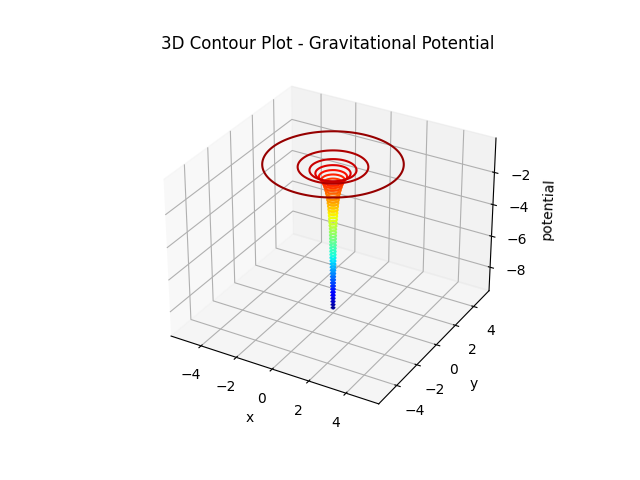
\includegraphics[width=0.4\columnwidth]{Figures/Figure4.png} 
		\caption[Final Physics 3D Contour Plot]{Final Physics 3D Contour Plot} % The text in the square bracket is the caption for the list of figures while the text in the curly brackets is the figure caption
		\label{fig:gallery} 
	\end{figure}

%----------------------------------------------------------------------------------------
%	BIBLIOGRAPHY
%----------------------------------------------------------------------------------------
\renewcommand{\refname}{\spacedlowsmallcaps{References}} % For modifying the bibliography heading
\raggedright
\bibliographystyle{unsrt}

\bibliography{sample.bib} % The file containing the bibliography

%----------------------------------------------------------------------------------------

\end{document}